\documentclass[1p]{elsarticle_modified}
%\bibliographystyle{elsarticle-num}

%\usepackage[colorlinks]{hyperref}
%\usepackage{abbrmath_seonhwa} %\Abb, \Ascr, \Acal ,\Abf, \Afrak
\usepackage{amsfonts}
\usepackage{amssymb}
\usepackage{amsmath}
\usepackage{amsthm}
\usepackage{scalefnt}
\usepackage{amsbsy}
\usepackage{kotex}
\usepackage{caption}
\usepackage{subfig}
\usepackage{color}
\usepackage{graphicx}
\usepackage{xcolor} %% white, black, red, green, blue, cyan, magenta, yellow
\usepackage{float}
\usepackage{setspace}
\usepackage{hyperref}

\usepackage{tikz}
\usetikzlibrary{arrows}

\usepackage{multirow}
\usepackage{array} % fixed length table
\usepackage{hhline}

%%%%%%%%%%%%%%%%%%%%%
\makeatletter
\renewcommand*\env@matrix[1][\arraystretch]{%
	\edef\arraystretch{#1}%
	\hskip -\arraycolsep
	\let\@ifnextchar\new@ifnextchar
	\array{*\c@MaxMatrixCols c}}
\makeatother %https://tex.stackexchange.com/questions/14071/how-can-i-increase-the-line-spacing-in-a-matrix
%%%%%%%%%%%%%%%

\usepackage[normalem]{ulem}

\newcommand{\msout}[1]{\ifmmode\text{\sout{\ensuremath{#1}}}\else\sout{#1}\fi}
%SOURCE: \msout is \stkout macro in https://tex.stackexchange.com/questions/20609/strikeout-in-math-mode

\newcommand{\cancel}[1]{
	\ifmmode
	{\color{red}\msout{#1}}
	\else
	{\color{red}\sout{#1}}
	\fi
}

\newcommand{\add}[1]{
	{\color{blue}\uwave{#1}}
}

\newcommand{\replace}[2]{
	\ifmmode
	{\color{red}\msout{#1}}{\color{blue}\uwave{#2}}
	\else
	{\color{red}\sout{#1}}{\color{blue}\uwave{#2}}
	\fi
}

\newcommand{\Sol}{\mathcal{S}} %segment
\newcommand{\D}{D} %diagram
\newcommand{\A}{\mathcal{A}} %arc


%%%%%%%%%%%%%%%%%%%%%%%%%%%%%5 test

\def\sl{\operatorname{\textup{SL}}(2,\Cbb)}
\def\psl{\operatorname{\textup{PSL}}(2,\Cbb)}
\def\quan{\mkern 1mu \triangleright \mkern 1mu}

\theoremstyle{definition}
\newtheorem{thm}{Theorem}[section]
\newtheorem{prop}[thm]{Proposition}
\newtheorem{lem}[thm]{Lemma}
\newtheorem{ques}[thm]{Question}
\newtheorem{cor}[thm]{Corollary}
\newtheorem{defn}[thm]{Definition}
\newtheorem{exam}[thm]{Example}
\newtheorem{rmk}[thm]{Remark}
\newtheorem{alg}[thm]{Algorithm}

\newcommand{\I}{\sqrt{-1}}
\begin{document}

%\begin{frontmatter}
%
%\title{Boundary parabolic representations of knots up to 8 crossings}
%
%%% Group authors per affiliation:
%\author{Yunhi Cho} 
%\address{Department of Mathematics, University of Seoul, Seoul, Korea}
%\ead{yhcho@uos.ac.kr}
%
%
%\author{Seonhwa Kim} %\fnref{s_kim}}
%\address{Center for Geometry and Physics, Institute for Basic Science, Pohang, 37673, Korea}
%\ead{ryeona17@ibs.re.kr}
%
%\author{Hyuk Kim}
%\address{Department of Mathematical Sciences, Seoul National University, Seoul 08826, Korea}
%\ead{hyukkim@snu.ac.kr}
%
%\author{Seokbeom Yoon}
%\address{Department of Mathematical Sciences, Seoul National University, Seoul, 08826,  Korea}
%\ead{sbyoon15@snu.ac.kr}
%
%\begin{abstract}
%We find all boundary parabolic representation of knots up to 8 crossings.
%
%\end{abstract}
%\begin{keyword}
%    \MSC[2010] 57M25 
%\end{keyword}
%
%\end{frontmatter}

%\linenumbers
%\tableofcontents
%
\newcommand\colored[1]{\textcolor{white}{\rule[-0.35ex]{0.8em}{1.4ex}}\kern-0.8em\color{red} #1}%
%\newcommand\colored[1]{\textcolor{white}{ #1}\kern-2.17ex	\textcolor{white}{ #1}\kern-1.81ex	\textcolor{white}{ #1}\kern-2.15ex\color{red}#1	}

{\Large $\underline{11a_{277}~(K11a_{277})}$}

\setlength{\tabcolsep}{10pt}
\renewcommand{\arraystretch}{1.6}
\vspace{1cm}\begin{tabular}{m{100pt}>{\centering\arraybackslash}m{274pt}}
\multirow{5}{120pt}{
	\centering
	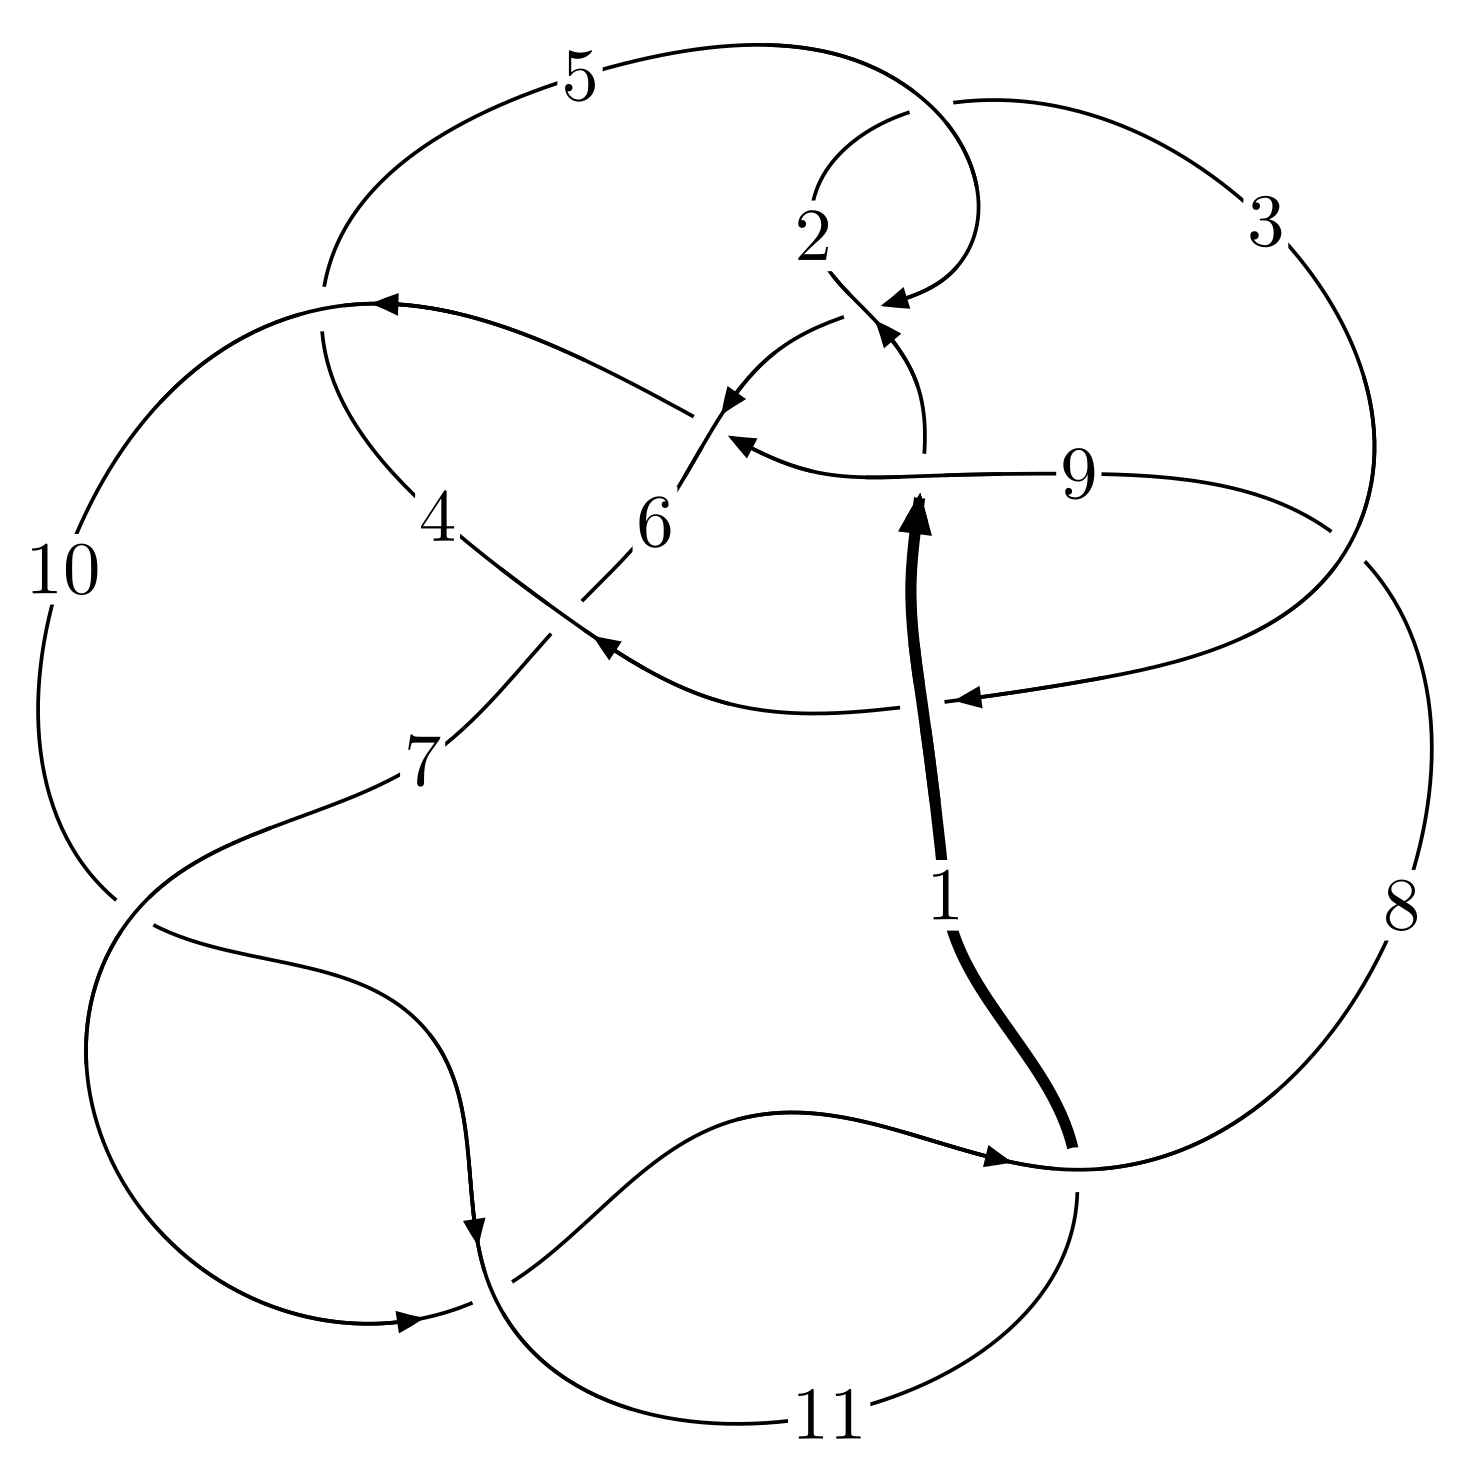
\includegraphics[width=112pt]{../../../GIT/diagram.site/Diagrams/png/526_11a_277.png}\\
\ \ \ A knot diagram\footnotemark}&
\allowdisplaybreaks
\textbf{Linearized knot diagam} \\
\cline{2-2}
 &
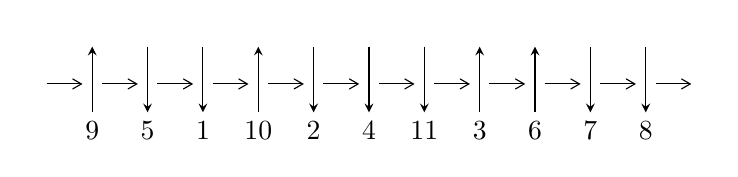
\begin{tikzpicture}[x=20pt, y=17pt]
	% nodes
	\node (C0) at (0, 0) {};
	\node (C1) at (1, 0) {};
	\node (C1U) at (1, +1) {};
	\node (C1D) at (1, -1) {9};

	\node (C2) at (2, 0) {};
	\node (C2U) at (2, +1) {};
	\node (C2D) at (2, -1) {5};

	\node (C3) at (3, 0) {};
	\node (C3U) at (3, +1) {};
	\node (C3D) at (3, -1) {1};

	\node (C4) at (4, 0) {};
	\node (C4U) at (4, +1) {};
	\node (C4D) at (4, -1) {10};

	\node (C5) at (5, 0) {};
	\node (C5U) at (5, +1) {};
	\node (C5D) at (5, -1) {2};

	\node (C6) at (6, 0) {};
	\node (C6U) at (6, +1) {};
	\node (C6D) at (6, -1) {4};

	\node (C7) at (7, 0) {};
	\node (C7U) at (7, +1) {};
	\node (C7D) at (7, -1) {11};

	\node (C8) at (8, 0) {};
	\node (C8U) at (8, +1) {};
	\node (C8D) at (8, -1) {3};

	\node (C9) at (9, 0) {};
	\node (C9U) at (9, +1) {};
	\node (C9D) at (9, -1) {6};

	\node (C10) at (10, 0) {};
	\node (C10U) at (10, +1) {};
	\node (C10D) at (10, -1) {7};

	\node (C11) at (11, 0) {};
	\node (C11U) at (11, +1) {};
	\node (C11D) at (11, -1) {8};
	\node (C12) at (12, 0) {};

	% arrows
	\draw[->,>={angle 60}]
	(C0) edge (C1) (C1) edge (C2) (C2) edge (C3) (C3) edge (C4) (C4) edge (C5) (C5) edge (C6) (C6) edge (C7) (C7) edge (C8) (C8) edge (C9) (C9) edge (C10) (C10) edge (C11) (C11) edge (C12) ;	\draw[->,>=stealth]
	(C1D) edge (C1U) (C2U) edge (C2D) (C3U) edge (C3D) (C4D) edge (C4U) (C5U) edge (C5D) (C6U) edge (C6D) (C7U) edge (C7D) (C8D) edge (C8U) (C9D) edge (C9U) (C10U) edge (C10D) (C11U) edge (C11D) ;
	\end{tikzpicture} \\
\hhline{~~} \\& 
\textbf{Solving Sequence} \\ \cline{2-2} 
 &
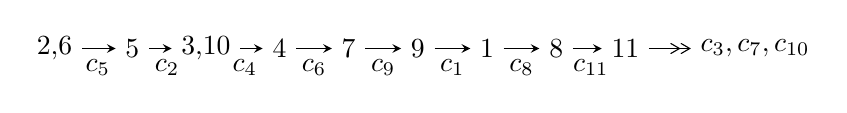
\begin{tikzpicture}[x=25pt, y=7pt]
	% node
	\node (A0) at (-1/8, 0) {2,6};
	\node (A1) at (1, 0) {5};
	\node (A2) at (33/16, 0) {3,10};
	\node (A3) at (25/8, 0) {4};
	\node (A4) at (33/8, 0) {7};
	\node (A5) at (41/8, 0) {9};
	\node (A6) at (49/8, 0) {1};
	\node (A7) at (57/8, 0) {8};
	\node (A8) at (65/8, 0) {11};
	\node (C1) at (1/2, -1) {$c_{5}$};
	\node (C2) at (3/2, -1) {$c_{2}$};
	\node (C3) at (21/8, -1) {$c_{4}$};
	\node (C4) at (29/8, -1) {$c_{6}$};
	\node (C5) at (37/8, -1) {$c_{9}$};
	\node (C6) at (45/8, -1) {$c_{1}$};
	\node (C7) at (53/8, -1) {$c_{8}$};
	\node (C8) at (61/8, -1) {$c_{11}$};
	\node (A9) at (10, 0) {$c_{3},c_{7},c_{10}$};

	% edge
	\draw[->,>=stealth]	
	(A0) edge (A1) (A1) edge (A2) (A2) edge (A3) (A3) edge (A4) (A4) edge (A5) (A5) edge (A6) (A6) edge (A7) (A7) edge (A8) ;
	\draw[->>,>={angle 60}]	
	(A8) edge (A9);
\end{tikzpicture} \\ 

\end{tabular} \\

\footnotetext{
The image of knot diagram is generated by the software ``\textbf{Draw programme}" developed by Andrew Bartholomew(\url{http://www.layer8.co.uk/maths/draw/index.htm\#Running-draw}), where we modified some parts for our purpose(\url{https://github.com/CATsTAILs/LinksPainter}).
}\phantom \\ \newline 
\centering \textbf{Ideals for irreducible components\footnotemark of $X_{\text{par}}$} 
 
\begin{align*}
I^u_{1}&=\langle 
-1.82122\times10^{22} u^{34}+1.39965\times10^{23} u^{33}+\cdots+1.46127\times10^{23} b+1.58974\times10^{23},\\
\phantom{I^u_{1}}&\phantom{= \langle  }-3.04671\times10^{23} u^{34}+2.69618\times10^{24} u^{33}+\cdots+1.16902\times10^{24} a-1.80715\times10^{25},\\
\phantom{I^u_{1}}&\phantom{= \langle  }u^{35}-9 u^{34}+\cdots+129 u-8\rangle \\
I^u_{2}&=\langle 
- u^{23} a- u^{23}+\cdots-3 a-1,\;4 u^{23} a- u^{23}+\cdots-18 a-11,\;u^{24}+7 u^{23}+\cdots+15 u+3\rangle \\
I^u_{3}&=\langle 
- u^{11}-6 u^{10}-20 u^9-46 u^8-76 u^7-94 u^6-86 u^5-57 u^4-28 u^3-11 u^2+b-5 u-1,\\
\phantom{I^u_{3}}&\phantom{= \langle  }- u^{10}-6 u^9-20 u^8-45 u^7-72 u^6-85 u^5-72 u^4-43 u^3-18 u^2+a-6 u-3,\\
\phantom{I^u_{3}}&\phantom{= \langle  }u^{12}+6 u^{11}+20 u^{10}+46 u^9+77 u^8+98 u^7+95 u^6+71 u^5+42 u^4+21 u^3+10 u^2+3 u+1\rangle \\
I^u_{4}&=\langle 
a u+2 b- a- u-1,\;a^2+a u- a-3 u-2,\;u^2+1\rangle \\
\\
\end{align*}
\raggedright * 4 irreducible components of $\dim_{\mathbb{C}}=0$, with total 99 representations.\\
\footnotetext{All coefficients of polynomials are rational numbers. But the coefficients are sometimes approximated in decimal forms when there is not enough margin.}
\newpage
\renewcommand{\arraystretch}{1}
\centering \section*{I. $I^u_{1}= \langle -1.82\times10^{22} u^{34}+1.40\times10^{23} u^{33}+\cdots+1.46\times10^{23} b+1.59\times10^{23},\;-3.05\times10^{23} u^{34}+2.70\times10^{24} u^{33}+\cdots+1.17\times10^{24} a-1.81\times10^{25},\;u^{35}-9 u^{34}+\cdots+129 u-8 \rangle$}
\flushleft \textbf{(i) Arc colorings}\\
\begin{tabular}{m{7pt} m{180pt} m{7pt} m{180pt} }
\flushright $a_{2}=$&$\begin{pmatrix}0\\u\end{pmatrix}$ \\
\flushright $a_{6}=$&$\begin{pmatrix}1\\0\end{pmatrix}$ \\
\flushright $a_{5}=$&$\begin{pmatrix}1\\- u^2\end{pmatrix}$ \\
\flushright $a_{3}=$&$\begin{pmatrix}- u\\u^3+u\end{pmatrix}$ \\
\flushright $a_{10}=$&$\begin{pmatrix}0.260621 u^{34}-2.30636 u^{33}+\cdots-109.860 u+15.4587\\0.124632 u^{34}-0.957827 u^{33}+\cdots+0.995973 u-1.08791\end{pmatrix}$ \\
\flushright $a_{4}=$&$\begin{pmatrix}0.0292774 u^{34}-0.335350 u^{33}+\cdots+46.0876 u-8.56756\\0.255676 u^{34}-2.11726 u^{33}+\cdots-17.8267 u+1.81119\end{pmatrix}$ \\
\flushright $a_{7}=$&$\begin{pmatrix}0.0652835 u^{34}-0.480129 u^{33}+\cdots+39.1684 u-5.24345\\0.0574092 u^{34}-0.366296 u^{33}+\cdots+9.72748 u-0.148606\end{pmatrix}$ \\
\flushright $a_{9}=$&$\begin{pmatrix}0.135989 u^{34}-1.34853 u^{33}+\cdots-110.856 u+16.5466\\0.124632 u^{34}-0.957827 u^{33}+\cdots+0.995973 u-1.08791\end{pmatrix}$ \\
\flushright $a_{1}=$&$\begin{pmatrix}0.0878378 u^{34}-0.551320 u^{33}+\cdots+70.1500 u-12.5898\\-0.239219 u^{34}+2.22799 u^{33}+\cdots+24.9209 u-0.702702\end{pmatrix}$ \\
\flushright $a_{8}=$&$\begin{pmatrix}0.0523471 u^{34}-0.798413 u^{33}+\cdots-122.147 u+17.1988\\0.207975 u^{34}-1.87903 u^{33}+\cdots-13.1866 u-0.118874\end{pmatrix}$ \\
\flushright $a_{11}=$&$\begin{pmatrix}-0.115771 u^{34}+1.07918 u^{33}+\cdots-32.8480 u+6.98223\\-0.0743855 u^{34}+0.536396 u^{33}+\cdots-12.8514 u+0.573324\end{pmatrix}$\\ \flushright $a_{11}=$&$\begin{pmatrix}-0.115771 u^{34}+1.07918 u^{33}+\cdots-32.8480 u+6.98223\\-0.0743855 u^{34}+0.536396 u^{33}+\cdots-12.8514 u+0.573324\end{pmatrix}$\\&\end{tabular}
\flushleft \textbf{(ii) Obstruction class $= -1$}\\~\\
\flushleft \textbf{(iii) Cusp Shapes $= \frac{90490086581286093778343}{146127200816312655174817} u^{34}-\frac{992059524318749332684051}{146127200816312655174817} u^{33}+\cdots-\frac{24335687627182500119507765}{146127200816312655174817} u+\frac{1325772668265518534675334}{146127200816312655174817}$}\\~\\
\newpage\renewcommand{\arraystretch}{1}
\flushleft \textbf{(iv) u-Polynomials at the component}\newline \\
\begin{tabular}{m{50pt}|m{274pt}}
Crossings & \hspace{64pt}u-Polynomials at each crossing \\
\hline $$\begin{aligned}c_{1},c_{9}\end{aligned}$$&$\begin{aligned}
&u^{35}+2 u^{34}+\cdots- u-1
\end{aligned}$\\
\hline $$\begin{aligned}c_{2},c_{5}\end{aligned}$$&$\begin{aligned}
&u^{35}-9 u^{34}+\cdots+129 u-8
\end{aligned}$\\
\hline $$\begin{aligned}c_{3},c_{6}\end{aligned}$$&$\begin{aligned}
&u^{35}-2 u^{34}+\cdots-7 u-2
\end{aligned}$\\
\hline $$\begin{aligned}c_{4},c_{8}\end{aligned}$$&$\begin{aligned}
&u^{35}+5 u^{33}+\cdots-10 u-4
\end{aligned}$\\
\hline $$\begin{aligned}c_{7},c_{10},c_{11}\end{aligned}$$&$\begin{aligned}
&u^{35}+10 u^{34}+\cdots-7 u-2
\end{aligned}$\\
\hline
\end{tabular}\\~\\
\newpage\renewcommand{\arraystretch}{1}
\flushleft \textbf{(v) Riley Polynomials at the component}\newline \\
\begin{tabular}{m{50pt}|m{274pt}}
Crossings & \hspace{64pt}Riley Polynomials at each crossing \\
\hline $$\begin{aligned}c_{1},c_{9}\end{aligned}$$&$\begin{aligned}
&y^{35}-28 y^{34}+\cdots+97 y-1
\end{aligned}$\\
\hline $$\begin{aligned}c_{2},c_{5}\end{aligned}$$&$\begin{aligned}
&y^{35}+17 y^{34}+\cdots+5825 y-64
\end{aligned}$\\
\hline $$\begin{aligned}c_{3},c_{6}\end{aligned}$$&$\begin{aligned}
&y^{35}+4 y^{34}+\cdots-35 y-4
\end{aligned}$\\
\hline $$\begin{aligned}c_{4},c_{8}\end{aligned}$$&$\begin{aligned}
&y^{35}+10 y^{34}+\cdots-68 y-16
\end{aligned}$\\
\hline $$\begin{aligned}c_{7},c_{10},c_{11}\end{aligned}$$&$\begin{aligned}
&y^{35}-38 y^{34}+\cdots-63 y-4
\end{aligned}$\\
\hline
\end{tabular}\\~\\
\newpage\flushleft \textbf{(vi) Complex Volumes and Cusp Shapes}
$$\begin{array}{c|c|c}  
\text{Solutions to }I^u_{1}& \I (\text{vol} + \sqrt{-1}CS) & \text{Cusp shape}\\
 \hline 
\begin{aligned}
u &= -0.029467 + 1.005660 I \\
a &= \phantom{-}1.62337 + 0.62304 I \\
b &= \phantom{-}1.118990 - 0.474878 I\end{aligned}
 & \phantom{-}3.33325 + 0.06783 I & \phantom{-}5.95235 + 0.12495 I \\ \hline\begin{aligned}
u &= -0.029467 - 1.005660 I \\
a &= \phantom{-}1.62337 - 0.62304 I \\
b &= \phantom{-}1.118990 + 0.474878 I\end{aligned}
 & \phantom{-}3.33325 - 0.06783 I & \phantom{-}5.95235 - 0.12495 I \\ \hline\begin{aligned}
u &= -0.160155 + 0.940171 I \\
a &= -1.89608 - 0.73160 I \\
b &= -1.218050 + 0.448463 I\end{aligned}
 & -1.89744 + 0.70933 I & -2.29610 + 0.18489 I \\ \hline\begin{aligned}
u &= -0.160155 - 0.940171 I \\
a &= -1.89608 + 0.73160 I \\
b &= -1.218050 - 0.448463 I\end{aligned}
 & -1.89744 - 0.70933 I & -2.29610 - 0.18489 I \\ \hline\begin{aligned}
u &= \phantom{-}1.032060 + 0.216151 I \\
a &= \phantom{-}0.065858 - 0.238657 I \\
b &= -0.970266 - 0.697041 I\end{aligned}
 & -0.31706 + 7.01027 I & -3.82014 - 7.79890 I \\ \hline\begin{aligned}
u &= \phantom{-}1.032060 - 0.216151 I \\
a &= \phantom{-}0.065858 + 0.238657 I \\
b &= -0.970266 + 0.697041 I\end{aligned}
 & -0.31706 - 7.01027 I & -3.82014 + 7.79890 I \\ \hline\begin{aligned}
u &= \phantom{-}0.030627 + 1.114570 I \\
a &= -1.64670 - 0.23881 I \\
b &= -1.037110 + 0.708446 I\end{aligned}
 & -0.301669 - 0.553139 I & -3.58187 + 1.60443 I \\ \hline\begin{aligned}
u &= \phantom{-}0.030627 - 1.114570 I \\
a &= -1.64670 + 0.23881 I \\
b &= -1.037110 - 0.708446 I\end{aligned}
 & -0.301669 + 0.553139 I & -3.58187 - 1.60443 I \\ \hline\begin{aligned}
u &= -1.11586\phantom{ +0.000000I} \\
a &= -0.236593\phantom{ +0.000000I} \\
b &= -0.124774\phantom{ +0.000000I}\end{aligned}
 & -2.17258\phantom{ +0.000000I} & -20.5000\phantom{ +0.000000I} \\ \hline\begin{aligned}
u &= \phantom{-}0.746671 + 0.829900 I \\
a &= -0.135819 - 1.208780 I \\
b &= -1.42250 - 0.65236 I\end{aligned}
 & -5.09357 - 3.39425 I & -14.2242 + 15.5417 I\\
 \hline 
 \end{array}$$\newpage$$\begin{array}{c|c|c}  
\text{Solutions to }I^u_{1}& \I (\text{vol} + \sqrt{-1}CS) & \text{Cusp shape}\\
 \hline 
\begin{aligned}
u &= \phantom{-}0.746671 - 0.829900 I \\
a &= -0.135819 + 1.208780 I \\
b &= -1.42250 + 0.65236 I\end{aligned}
 & -5.09357 + 3.39425 I & -14.2242 - 15.5417 I \\ \hline\begin{aligned}
u &= \phantom{-}0.648498 + 0.961930 I \\
a &= -1.22988 - 0.79688 I \\
b &= -1.54855 + 0.59812 I\end{aligned}
 & -4.64663 - 2.02674 I & -10.39702 - 3.31188 I \\ \hline\begin{aligned}
u &= \phantom{-}0.648498 - 0.961930 I \\
a &= -1.22988 + 0.79688 I \\
b &= -1.54855 - 0.59812 I\end{aligned}
 & -4.64663 + 2.02674 I & -10.39702 + 3.31188 I \\ \hline\begin{aligned}
u &= -0.795787 + 0.881934 I \\
a &= \phantom{-}0.657988 - 0.155281 I \\
b &= \phantom{-}0.328568 - 0.230594 I\end{aligned}
 & -6.54898 + 2.97371 I & -10.02830 - 2.31900 I \\ \hline\begin{aligned}
u &= -0.795787 - 0.881934 I \\
a &= \phantom{-}0.657988 + 0.155281 I \\
b &= \phantom{-}0.328568 + 0.230594 I\end{aligned}
 & -6.54898 - 2.97371 I & -10.02830 + 2.31900 I \\ \hline\begin{aligned}
u &= \phantom{-}0.405669 + 1.141420 I \\
a &= \phantom{-}0.894751 + 0.750550 I \\
b &= \phantom{-}1.090950 - 0.135501 I\end{aligned}
 & \phantom{-}4.39987 - 1.11837 I & \phantom{-}2.66422 + 2.51524 I \\ \hline\begin{aligned}
u &= \phantom{-}0.405669 - 1.141420 I \\
a &= \phantom{-}0.894751 - 0.750550 I \\
b &= \phantom{-}1.090950 + 0.135501 I\end{aligned}
 & \phantom{-}4.39987 + 1.11837 I & \phantom{-}2.66422 - 2.51524 I \\ \hline\begin{aligned}
u &= \phantom{-}0.719504 + 0.276631 I \\
a &= -0.532660 + 0.260522 I \\
b &= \phantom{-}0.894361 + 0.739088 I\end{aligned}
 & \phantom{-}0.64524 + 2.18197 I & -1.66363 - 5.31437 I \\ \hline\begin{aligned}
u &= \phantom{-}0.719504 - 0.276631 I \\
a &= -0.532660 - 0.260522 I \\
b &= \phantom{-}0.894361 - 0.739088 I\end{aligned}
 & \phantom{-}0.64524 - 2.18197 I & -1.66363 + 5.31437 I \\ \hline\begin{aligned}
u &= \phantom{-}1.204480 + 0.248072 I \\
a &= \phantom{-}0.084193 + 0.300543 I \\
b &= \phantom{-}0.972158 + 0.693076 I\end{aligned}
 & -7.58044 + 10.41690 I & -6.58450 - 6.84896 I\\
 \hline 
 \end{array}$$\newpage$$\begin{array}{c|c|c}  
\text{Solutions to }I^u_{1}& \I (\text{vol} + \sqrt{-1}CS) & \text{Cusp shape}\\
 \hline 
\begin{aligned}
u &= \phantom{-}1.204480 - 0.248072 I \\
a &= \phantom{-}0.084193 - 0.300543 I \\
b &= \phantom{-}0.972158 - 0.693076 I\end{aligned}
 & -7.58044 - 10.41690 I & -6.58450 + 6.84896 I \\ \hline\begin{aligned}
u &= \phantom{-}0.548826 + 1.162060 I \\
a &= \phantom{-}1.67262 + 0.38811 I \\
b &= \phantom{-}1.47723 - 0.97539 I\end{aligned}
 & \phantom{-}3.22979 - 7.07568 I & -1.38313 + 9.02703 I \\ \hline\begin{aligned}
u &= \phantom{-}0.548826 - 1.162060 I \\
a &= \phantom{-}1.67262 - 0.38811 I \\
b &= \phantom{-}1.47723 + 0.97539 I\end{aligned}
 & \phantom{-}3.22979 + 7.07568 I & -1.38313 - 9.02703 I \\ \hline\begin{aligned}
u &= -0.308052 + 0.545459 I \\
a &= -0.928218 + 0.582030 I \\
b &= -0.165653 + 0.455061 I\end{aligned}
 & -0.241930 + 1.296500 I & -3.54219 - 4.67694 I \\ \hline\begin{aligned}
u &= -0.308052 - 0.545459 I \\
a &= -0.928218 - 0.582030 I \\
b &= -0.165653 - 0.455061 I\end{aligned}
 & -0.241930 - 1.296500 I & -3.54219 + 4.67694 I \\ \hline\begin{aligned}
u &= \phantom{-}0.271698 + 1.365610 I \\
a &= -0.854456 - 0.533102 I \\
b &= -0.898585 + 0.116131 I\end{aligned}
 & \phantom{-}5.18517 + 2.44630 I & \phantom{-0.000000 } 0. - 4.73123 I \\ \hline\begin{aligned}
u &= \phantom{-}0.271698 - 1.365610 I \\
a &= -0.854456 + 0.533102 I \\
b &= -0.898585 - 0.116131 I\end{aligned}
 & \phantom{-}5.18517 - 2.44630 I & \phantom{-0.000000 -}0. + 4.73123 I \\ \hline\begin{aligned}
u &= \phantom{-}0.595757 + 1.264360 I \\
a &= -1.58942 - 0.26495 I \\
b &= -1.41489 + 0.93635 I\end{aligned}
 & \phantom{-}2.94252 - 12.83480 I & \phantom{-0.000000 -}0. + 9.50250 I \\ \hline\begin{aligned}
u &= \phantom{-}0.595757 - 1.264360 I \\
a &= -1.58942 + 0.26495 I \\
b &= -1.41489 - 0.93635 I\end{aligned}
 & \phantom{-}2.94252 + 12.83480 I & \phantom{-0.000000 } 0. - 9.50250 I \\ \hline\begin{aligned}
u &= -1.41303\phantom{ +0.000000I} \\
a &= \phantom{-}0.370029\phantom{ +0.000000I} \\
b &= \phantom{-}0.216683\phantom{ +0.000000I}\end{aligned}
 & -8.46698\phantom{ +0.000000I} & -18.1290\phantom{ +0.000000I}\\
 \hline 
 \end{array}$$\newpage$$\begin{array}{c|c|c}  
\text{Solutions to }I^u_{1}& \I (\text{vol} + \sqrt{-1}CS) & \text{Cusp shape}\\
 \hline 
\begin{aligned}
u &= \phantom{-}0.64890 + 1.31702 I \\
a &= \phantom{-}1.53917 + 0.20834 I \\
b &= \phantom{-}1.39598 - 0.92217 I\end{aligned}
 & -4.1620 - 16.9207 I & \phantom{-0.000000 } 0 \\ \hline\begin{aligned}
u &= \phantom{-}0.64890 - 1.31702 I \\
a &= \phantom{-}1.53917 - 0.20834 I \\
b &= \phantom{-}1.39598 + 0.92217 I\end{aligned}
 & -4.1620 + 16.9207 I & \phantom{-0.000000 } 0 \\ \hline\begin{aligned}
u &= \phantom{-}0.15479 + 1.53945 I \\
a &= \phantom{-}0.793512 + 0.415691 I \\
b &= \phantom{-}0.783542 - 0.094287 I\end{aligned}
 & -0.87578 + 5.04274 I & \phantom{-0.000000 } 0 \\ \hline\begin{aligned}
u &= \phantom{-}0.15479 - 1.53945 I \\
a &= \phantom{-}0.793512 - 0.415691 I \\
b &= \phantom{-}0.783542 + 0.094287 I\end{aligned}
 & -0.87578 - 5.04274 I & \phantom{-0.000000 } 0 \\ \hline\begin{aligned}
u &= \phantom{-}0.100849\phantom{ +0.000000I} \\
a &= \phantom{-}7.70512\phantom{ +0.000000I} \\
b &= -0.864213\phantom{ +0.000000I}\end{aligned}
 & -3.33456\phantom{ +0.000000I} & -1.41010\phantom{ +0.000000I}\\
 \hline 
 \end{array}$$\newpage\newpage\renewcommand{\arraystretch}{1}
\centering \section*{II. $I^u_{2}= \langle - u^{23} a- u^{23}+\cdots-3 a-1,\;4 u^{23} a- u^{23}+\cdots-18 a-11,\;u^{24}+7 u^{23}+\cdots+15 u+3 \rangle$}
\flushleft \textbf{(i) Arc colorings}\\
\begin{tabular}{m{7pt} m{180pt} m{7pt} m{180pt} }
\flushright $a_{2}=$&$\begin{pmatrix}0\\u\end{pmatrix}$ \\
\flushright $a_{6}=$&$\begin{pmatrix}1\\0\end{pmatrix}$ \\
\flushright $a_{5}=$&$\begin{pmatrix}1\\- u^2\end{pmatrix}$ \\
\flushright $a_{3}=$&$\begin{pmatrix}- u\\u^3+u\end{pmatrix}$ \\
\flushright $a_{10}=$&$\begin{pmatrix}a\\\frac{1}{2} u^{23} a+\frac{1}{2} u^{23}+\cdots+\frac{3}{2} a+\frac{1}{2}\end{pmatrix}$ \\
\flushright $a_{4}=$&$\begin{pmatrix}\frac{1}{2} u^{23} a+\frac{1}{6} u^{23}+\cdots+\frac{3}{2} a-\frac{3}{2}\\- u^{23} a-6 u^{22} a+\cdots+u-1\end{pmatrix}$ \\
\flushright $a_{7}=$&$\begin{pmatrix}\frac{1}{2} u^{23} a+\frac{5}{6} u^{23}+\cdots+\frac{1}{2} a+\frac{7}{2}\\u^{23} a+7 u^{22} a+\cdots+3 a-1\end{pmatrix}$ \\
\flushright $a_{9}=$&$\begin{pmatrix}-\frac{1}{2} u^{23} a-\frac{1}{2} u^{23}+\cdots-\frac{1}{2} a-\frac{1}{2}\\\frac{1}{2} u^{23} a+\frac{1}{2} u^{23}+\cdots+\frac{3}{2} a+\frac{1}{2}\end{pmatrix}$ \\
\flushright $a_{1}=$&$\begin{pmatrix}\frac{1}{2} u^{23} a+\frac{5}{6} u^{23}+\cdots+\frac{1}{2} a+\frac{9}{2}\\-1\end{pmatrix}$ \\
\flushright $a_{8}=$&$\begin{pmatrix}u^{23}+8 u^{22}+\cdots+a-2\\-\frac{1}{2} u^{23} a+\frac{1}{2} u^{23}+\cdots-\frac{3}{2} a+\frac{1}{2}\end{pmatrix}$ \\
\flushright $a_{11}=$&$\begin{pmatrix}\frac{1}{2} u^{23} a+\frac{5}{6} u^{23}+\cdots+\frac{3}{2} a+\frac{5}{2}\\\frac{1}{2} u^{23} a+\frac{1}{2} u^{23}+\cdots+\frac{3}{2} a-\frac{1}{2}\end{pmatrix}$\\ \flushright $a_{11}=$&$\begin{pmatrix}\frac{1}{2} u^{23} a+\frac{5}{6} u^{23}+\cdots+\frac{3}{2} a+\frac{5}{2}\\\frac{1}{2} u^{23} a+\frac{1}{2} u^{23}+\cdots+\frac{3}{2} a-\frac{1}{2}\end{pmatrix}$\\&\end{tabular}
\flushleft \textbf{(ii) Obstruction class $= -1$}\\~\\
\flushleft \textbf{(iii) Cusp Shapes $= -2 u^{23}-10 u^{22}-38 u^{21}-96 u^{20}-196 u^{19}-310 u^{18}-390 u^{17}-364 u^{16}-176 u^{15}+152 u^{14}+576 u^{13}+960 u^{12}+1228 u^{11}+1294 u^{10}+1190 u^9+956 u^8+698 u^7+454 u^6+254 u^5+136 u^4+48 u^3+26 u^2+2 u-6$}\\~\\
\newpage\renewcommand{\arraystretch}{1}
\flushleft \textbf{(iv) u-Polynomials at the component}\newline \\
\begin{tabular}{m{50pt}|m{274pt}}
Crossings & \hspace{64pt}u-Polynomials at each crossing \\
\hline $$\begin{aligned}c_{1},c_{9}\end{aligned}$$&$\begin{aligned}
&u^{48}+u^{47}+\cdots+16 u^2+2
\end{aligned}$\\
\hline $$\begin{aligned}c_{2},c_{5}\end{aligned}$$&$\begin{aligned}
&(u^{24}+7 u^{23}+\cdots+15 u+3)^{2}
\end{aligned}$\\
\hline $$\begin{aligned}c_{3},c_{6}\end{aligned}$$&$\begin{aligned}
&u^{48}-7 u^{47}+\cdots-28 u+8
\end{aligned}$\\
\hline $$\begin{aligned}c_{4},c_{8}\end{aligned}$$&$\begin{aligned}
&u^{48}+u^{47}+\cdots-48 u+32
\end{aligned}$\\
\hline $$\begin{aligned}c_{7},c_{10},c_{11}\end{aligned}$$&$\begin{aligned}
&(u^{24}-3 u^{23}+\cdots+3 u-1)^{2}
\end{aligned}$\\
\hline
\end{tabular}\\~\\
\newpage\renewcommand{\arraystretch}{1}
\flushleft \textbf{(v) Riley Polynomials at the component}\newline \\
\begin{tabular}{m{50pt}|m{274pt}}
Crossings & \hspace{64pt}Riley Polynomials at each crossing \\
\hline $$\begin{aligned}c_{1},c_{9}\end{aligned}$$&$\begin{aligned}
&y^{48}+y^{47}+\cdots+64 y+4
\end{aligned}$\\
\hline $$\begin{aligned}c_{2},c_{5}\end{aligned}$$&$\begin{aligned}
&(y^{24}+15 y^{23}+\cdots+69 y+9)^{2}
\end{aligned}$\\
\hline $$\begin{aligned}c_{3},c_{6}\end{aligned}$$&$\begin{aligned}
&y^{48}-21 y^{47}+\cdots+176 y+64
\end{aligned}$\\
\hline $$\begin{aligned}c_{4},c_{8}\end{aligned}$$&$\begin{aligned}
&y^{48}+9 y^{47}+\cdots+20736 y+1024
\end{aligned}$\\
\hline $$\begin{aligned}c_{7},c_{10},c_{11}\end{aligned}$$&$\begin{aligned}
&(y^{24}-25 y^{23}+\cdots-15 y+1)^{2}
\end{aligned}$\\
\hline
\end{tabular}\\~\\
\newpage\flushleft \textbf{(vi) Complex Volumes and Cusp Shapes}
$$\begin{array}{c|c|c}  
\text{Solutions to }I^u_{2}& \I (\text{vol} + \sqrt{-1}CS) & \text{Cusp shape}\\
 \hline 
\begin{aligned}
u &= \phantom{-}0.333614 + 0.958581 I \\
a &= \phantom{-}0.238717 + 0.952089 I \\
b &= \phantom{-}0.52014 + 1.77867 I\end{aligned}
 & -7.10793 - 8.02681 I & -5.10804 + 8.04729 I \\ \hline\begin{aligned}
u &= \phantom{-}0.333614 + 0.958581 I \\
a &= -2.52196 + 0.45351 I \\
b &= -0.698461 + 0.545528 I\end{aligned}
 & -7.10793 - 8.02681 I & -5.10804 + 8.04729 I \\ \hline\begin{aligned}
u &= \phantom{-}0.333614 - 0.958581 I \\
a &= \phantom{-}0.238717 - 0.952089 I \\
b &= \phantom{-}0.52014 - 1.77867 I\end{aligned}
 & -7.10793 + 8.02681 I & -5.10804 - 8.04729 I \\ \hline\begin{aligned}
u &= \phantom{-}0.333614 - 0.958581 I \\
a &= -2.52196 - 0.45351 I \\
b &= -0.698461 - 0.545528 I\end{aligned}
 & -7.10793 + 8.02681 I & -5.10804 - 8.04729 I \\ \hline\begin{aligned}
u &= -1.06754\phantom{ +0.000000I} \\
a &= -0.247659 + 0.014314 I \\
b &= -0.127875 + 0.226247 I\end{aligned}
 & -2.16765\phantom{ +0.000000I} & -17.3620\phantom{ +0.000000I} \\ \hline\begin{aligned}
u &= -1.06754\phantom{ +0.000000I} \\
a &= -0.247659 - 0.014314 I \\
b &= -0.127875 - 0.226247 I\end{aligned}
 & -2.16765\phantom{ +0.000000I} & -17.3620\phantom{ +0.000000I} \\ \hline\begin{aligned}
u &= -0.277461 + 1.036230 I \\
a &= \phantom{-}0.412312 - 1.328630 I \\
b &= \phantom{-}0.487830 + 0.447909 I\end{aligned}
 & \phantom{-}1.42987 + 1.40919 I & -2.00295 - 5.17297 I \\ \hline\begin{aligned}
u &= -0.277461 + 1.036230 I \\
a &= -2.14757 + 0.13261 I \\
b &= -1.86186 - 0.41467 I\end{aligned}
 & \phantom{-}1.42987 + 1.40919 I & -2.00295 - 5.17297 I \\ \hline\begin{aligned}
u &= -0.277461 - 1.036230 I \\
a &= \phantom{-}0.412312 + 1.328630 I \\
b &= \phantom{-}0.487830 - 0.447909 I\end{aligned}
 & \phantom{-}1.42987 - 1.40919 I & -2.00295 + 5.17297 I \\ \hline\begin{aligned}
u &= -0.277461 - 1.036230 I \\
a &= -2.14757 - 0.13261 I \\
b &= -1.86186 + 0.41467 I\end{aligned}
 & \phantom{-}1.42987 - 1.40919 I & -2.00295 + 5.17297 I\\
 \hline 
 \end{array}$$\newpage$$\begin{array}{c|c|c}  
\text{Solutions to }I^u_{2}& \I (\text{vol} + \sqrt{-1}CS) & \text{Cusp shape}\\
 \hline 
\begin{aligned}
u &= \phantom{-}0.263524 + 0.887339 I \\
a &= \phantom{-}0.252966 - 0.916113 I \\
b &= -0.23360 - 1.73518 I\end{aligned}
 & -0.45153 - 3.90914 I & -4.05947 + 8.41437 I \\ \hline\begin{aligned}
u &= \phantom{-}0.263524 + 0.887339 I \\
a &= \phantom{-}2.46741 - 0.35585 I \\
b &= \phantom{-}0.598566 - 0.647596 I\end{aligned}
 & -0.45153 - 3.90914 I & -4.05947 + 8.41437 I \\ \hline\begin{aligned}
u &= \phantom{-}0.263524 - 0.887339 I \\
a &= \phantom{-}0.252966 + 0.916113 I \\
b &= -0.23360 + 1.73518 I\end{aligned}
 & -0.45153 + 3.90914 I & -4.05947 - 8.41437 I \\ \hline\begin{aligned}
u &= \phantom{-}0.263524 - 0.887339 I \\
a &= \phantom{-}2.46741 + 0.35585 I \\
b &= \phantom{-}0.598566 + 0.647596 I\end{aligned}
 & -0.45153 + 3.90914 I & -4.05947 - 8.41437 I \\ \hline\begin{aligned}
u &= -0.887982 + 0.619939 I \\
a &= \phantom{-}0.994897 - 0.465007 I \\
b &= \phantom{-}0.852325 + 0.186324 I\end{aligned}
 & -6.92221 + 3.07969 I & -9.61105 - 4.95105 I \\ \hline\begin{aligned}
u &= -0.887982 + 0.619939 I \\
a &= \phantom{-}0.269644 - 0.075164 I \\
b &= -0.277184 - 0.666756 I\end{aligned}
 & -6.92221 + 3.07969 I & -9.61105 - 4.95105 I \\ \hline\begin{aligned}
u &= -0.887982 - 0.619939 I \\
a &= \phantom{-}0.994897 + 0.465007 I \\
b &= \phantom{-}0.852325 - 0.186324 I\end{aligned}
 & -6.92221 - 3.07969 I & -9.61105 + 4.95105 I \\ \hline\begin{aligned}
u &= -0.887982 - 0.619939 I \\
a &= \phantom{-}0.269644 + 0.075164 I \\
b &= -0.277184 + 0.666756 I\end{aligned}
 & -6.92221 - 3.07969 I & -9.61105 + 4.95105 I \\ \hline\begin{aligned}
u &= \phantom{-}0.237103 + 0.737994 I \\
a &= -0.590664 - 0.004510 I \\
b &= \phantom{-}0.198307 + 1.243170 I\end{aligned}
 & -0.89648 + 1.35600 I & -6.20233 + 1.19503 I \\ \hline\begin{aligned}
u &= \phantom{-}0.237103 + 0.737994 I \\
a &= -2.33888 + 0.63109 I \\
b &= -0.733711 + 0.878083 I\end{aligned}
 & -0.89648 + 1.35600 I & -6.20233 + 1.19503 I\\
 \hline 
 \end{array}$$\newpage$$\begin{array}{c|c|c}  
\text{Solutions to }I^u_{2}& \I (\text{vol} + \sqrt{-1}CS) & \text{Cusp shape}\\
 \hline 
\begin{aligned}
u &= \phantom{-}0.237103 - 0.737994 I \\
a &= -0.590664 + 0.004510 I \\
b &= \phantom{-}0.198307 - 1.243170 I\end{aligned}
 & -0.89648 - 1.35600 I & -6.20233 - 1.19503 I \\ \hline\begin{aligned}
u &= \phantom{-}0.237103 - 0.737994 I \\
a &= -2.33888 - 0.63109 I \\
b &= -0.733711 - 0.878083 I\end{aligned}
 & -0.89648 - 1.35600 I & -6.20233 - 1.19503 I \\ \hline\begin{aligned}
u &= -1.24600\phantom{ +0.000000I} \\
a &= \phantom{-}0.424934 + 0.086154 I \\
b &= \phantom{-}0.235738 + 0.436377 I\end{aligned}
 & -8.40649\phantom{ +0.000000I} & -13.8590\phantom{ +0.000000I} \\ \hline\begin{aligned}
u &= -1.24600\phantom{ +0.000000I} \\
a &= \phantom{-}0.424934 - 0.086154 I \\
b &= \phantom{-}0.235738 - 0.436377 I\end{aligned}
 & -8.40649\phantom{ +0.000000I} & -13.8590\phantom{ +0.000000I} \\ \hline\begin{aligned}
u &= \phantom{-}0.387072 + 0.629729 I \\
a &= -0.214970 + 0.319082 I \\
b &= -0.514411 - 1.214470 I\end{aligned}
 & -8.06651 + 4.88076 I & -7.61294 - 0.00229 I \\ \hline\begin{aligned}
u &= \phantom{-}0.387072 + 0.629729 I \\
a &= \phantom{-}2.61397 - 0.51468 I \\
b &= \phantom{-}0.849819 - 0.782163 I\end{aligned}
 & -8.06651 + 4.88076 I & -7.61294 - 0.00229 I \\ \hline\begin{aligned}
u &= \phantom{-}0.387072 - 0.629729 I \\
a &= -0.214970 - 0.319082 I \\
b &= -0.514411 + 1.214470 I\end{aligned}
 & -8.06651 - 4.88076 I & -7.61294 + 0.00229 I \\ \hline\begin{aligned}
u &= \phantom{-}0.387072 - 0.629729 I \\
a &= \phantom{-}2.61397 + 0.51468 I \\
b &= \phantom{-}0.849819 + 0.782163 I\end{aligned}
 & -8.06651 - 4.88076 I & -7.61294 + 0.00229 I \\ \hline\begin{aligned}
u &= -0.334204 + 1.242180 I \\
a &= -1.064980 + 0.825666 I \\
b &= -0.715953 - 0.434854 I\end{aligned}
 & \phantom{-}4.15748 + 4.71846 I & \phantom{-}5.79042 - 6.26335 I \\ \hline\begin{aligned}
u &= -0.334204 + 1.242180 I \\
a &= \phantom{-}1.63098 + 0.22953 I \\
b &= \phantom{-}1.44914 + 0.85482 I\end{aligned}
 & \phantom{-}4.15748 + 4.71846 I & \phantom{-}5.79042 - 6.26335 I\\
 \hline 
 \end{array}$$\newpage$$\begin{array}{c|c|c}  
\text{Solutions to }I^u_{2}& \I (\text{vol} + \sqrt{-1}CS) & \text{Cusp shape}\\
 \hline 
\begin{aligned}
u &= -0.334204 - 1.242180 I \\
a &= -1.064980 - 0.825666 I \\
b &= -0.715953 + 0.434854 I\end{aligned}
 & \phantom{-}4.15748 - 4.71846 I & \phantom{-}5.79042 + 6.26335 I \\ \hline\begin{aligned}
u &= -0.334204 - 1.242180 I \\
a &= \phantom{-}1.63098 - 0.22953 I \\
b &= \phantom{-}1.44914 - 0.85482 I\end{aligned}
 & \phantom{-}4.15748 - 4.71846 I & \phantom{-}5.79042 + 6.26335 I \\ \hline\begin{aligned}
u &= -0.510133 + 0.304616 I \\
a &= -0.939645 + 0.262682 I \\
b &= \phantom{-}0.433520 + 0.540630 I\end{aligned}
 & -0.17657 + 1.63085 I & -4.99918 - 5.43978 I \\ \hline\begin{aligned}
u &= -0.510133 + 0.304616 I \\
a &= -0.62521 + 1.43179 I \\
b &= -0.785164 + 0.276497 I\end{aligned}
 & -0.17657 + 1.63085 I & -4.99918 - 5.43978 I \\ \hline\begin{aligned}
u &= -0.510133 - 0.304616 I \\
a &= -0.939645 - 0.262682 I \\
b &= \phantom{-}0.433520 - 0.540630 I\end{aligned}
 & -0.17657 - 1.63085 I & -4.99918 + 5.43978 I \\ \hline\begin{aligned}
u &= -0.510133 - 0.304616 I \\
a &= -0.62521 - 1.43179 I \\
b &= -0.785164 - 0.276497 I\end{aligned}
 & -0.17657 - 1.63085 I & -4.99918 + 5.43978 I \\ \hline\begin{aligned}
u &= -0.54684 + 1.32589 I \\
a &= \phantom{-}0.913096 - 0.034885 I \\
b &= \phantom{-}0.839736 + 0.802838 I\end{aligned}
 & \phantom{-}1.92307 + 5.70686 I & -7.16158 - 11.30466 I \\ \hline\begin{aligned}
u &= -0.54684 + 1.32589 I \\
a &= -1.364860 + 0.199330 I \\
b &= -1.070610 - 0.555366 I\end{aligned}
 & \phantom{-}1.92307 + 5.70686 I & -7.16158 - 11.30466 I \\ \hline\begin{aligned}
u &= -0.54684 - 1.32589 I \\
a &= \phantom{-}0.913096 + 0.034885 I \\
b &= \phantom{-}0.839736 - 0.802838 I\end{aligned}
 & \phantom{-}1.92307 - 5.70686 I & -7.16158 + 11.30466 I \\ \hline\begin{aligned}
u &= -0.54684 - 1.32589 I \\
a &= -1.364860 - 0.199330 I \\
b &= -1.070610 + 0.555366 I\end{aligned}
 & \phantom{-}1.92307 - 5.70686 I & -7.16158 + 11.30466 I\\
 \hline 
 \end{array}$$\newpage$$\begin{array}{c|c|c}  
\text{Solutions to }I^u_{2}& \I (\text{vol} + \sqrt{-1}CS) & \text{Cusp shape}\\
 \hline 
\begin{aligned}
u &= -0.34545 + 1.40335 I \\
a &= -1.311200 - 0.410770 I \\
b &= -1.20101 - 1.06820 I\end{aligned}
 & -0.65429 + 7.12209 I & \phantom{-}0.24406 - 7.53717 I \\ \hline\begin{aligned}
u &= -0.34545 + 1.40335 I \\
a &= \phantom{-}1.40359 - 0.60184 I \\
b &= \phantom{-}0.884534 + 0.381753 I\end{aligned}
 & -0.65429 + 7.12209 I & \phantom{-}0.24406 - 7.53717 I \\ \hline\begin{aligned}
u &= -0.34545 - 1.40335 I \\
a &= -1.311200 + 0.410770 I \\
b &= -1.20101 + 1.06820 I\end{aligned}
 & -0.65429 - 7.12209 I & \phantom{-}0.24406 + 7.53717 I \\ \hline\begin{aligned}
u &= -0.34545 - 1.40335 I \\
a &= \phantom{-}1.40359 + 0.60184 I \\
b &= \phantom{-}0.884534 - 0.381753 I\end{aligned}
 & -0.65429 - 7.12209 I & \phantom{-}0.24406 + 7.53717 I \\ \hline\begin{aligned}
u &= -0.66247 + 1.36339 I \\
a &= -0.691207 - 0.146838 I \\
b &= -0.720461 - 0.932573 I\end{aligned}
 & -4.26677 + 6.65894 I & -7.66647 - 7.55605 I \\ \hline\begin{aligned}
u &= -0.66247 + 1.36339 I \\
a &= \phantom{-}1.43628 - 0.21574 I \\
b &= \phantom{-}1.090640 + 0.480643 I\end{aligned}
 & -4.26677 + 6.65894 I & -7.66647 - 7.55605 I \\ \hline\begin{aligned}
u &= -0.66247 - 1.36339 I \\
a &= -0.691207 + 0.146838 I \\
b &= -0.720461 + 0.932573 I\end{aligned}
 & -4.26677 - 6.65894 I & -7.66647 + 7.55605 I \\ \hline\begin{aligned}
u &= -0.66247 - 1.36339 I \\
a &= \phantom{-}1.43628 + 0.21574 I \\
b &= \phantom{-}1.090640 - 0.480643 I\end{aligned}
 & -4.26677 - 6.65894 I & -7.66647 + 7.55605 I\\
 \hline 
 \end{array}$$\newpage\newpage\renewcommand{\arraystretch}{1}
\centering \section*{III. $I^u_{3}= \langle - u^{11}-6 u^{10}+\cdots+b-1,\;- u^{10}-6 u^9+\cdots+a-3,\;u^{12}+6 u^{11}+\cdots+3 u+1 \rangle$}
\flushleft \textbf{(i) Arc colorings}\\
\begin{tabular}{m{7pt} m{180pt} m{7pt} m{180pt} }
\flushright $a_{2}=$&$\begin{pmatrix}0\\u\end{pmatrix}$ \\
\flushright $a_{6}=$&$\begin{pmatrix}1\\0\end{pmatrix}$ \\
\flushright $a_{5}=$&$\begin{pmatrix}1\\- u^2\end{pmatrix}$ \\
\flushright $a_{3}=$&$\begin{pmatrix}- u\\u^3+u\end{pmatrix}$ \\
\flushright $a_{10}=$&$\begin{pmatrix}u^{10}+6 u^9+\cdots+6 u+3\\u^{11}+6 u^{10}+\cdots+5 u+1\end{pmatrix}$ \\
\flushright $a_{4}=$&$\begin{pmatrix}u^{11}+6 u^{10}+\cdots+9 u+2\\- u^2- u-1\end{pmatrix}$ \\
\flushright $a_{7}=$&$\begin{pmatrix}- u^{11}-6 u^{10}+\cdots-19 u^2-7 u\\u^4+2 u^3+3 u^2+2 u+1\end{pmatrix}$ \\
\flushright $a_{9}=$&$\begin{pmatrix}- u^{11}-5 u^{10}+\cdots+u+2\\u^{11}+6 u^{10}+\cdots+5 u+1\end{pmatrix}$ \\
\flushright $a_{1}=$&$\begin{pmatrix}- u^{11}-7 u^{10}+\cdots-13 u-4\\- u^{11}-5 u^{10}+\cdots-3 u^2+1\end{pmatrix}$ \\
\flushright $a_{8}=$&$\begin{pmatrix}- u^{11}-4 u^{10}+\cdots+4 u+3\\2 u^{11}+11 u^{10}+\cdots+5 u+1\end{pmatrix}$ \\
\flushright $a_{11}=$&$\begin{pmatrix}- u^{11}-6 u^{10}+\cdots-8 u-1\\u^8+3 u^7+6 u^6+8 u^5+7 u^4+6 u^3+4 u^2+3 u+1\end{pmatrix}$\\ \flushright $a_{11}=$&$\begin{pmatrix}- u^{11}-6 u^{10}+\cdots-8 u-1\\u^8+3 u^7+6 u^6+8 u^5+7 u^4+6 u^3+4 u^2+3 u+1\end{pmatrix}$\\&\end{tabular}
\flushleft \textbf{(ii) Obstruction class $= 1$}\\~\\
\flushleft \textbf{(iii) Cusp Shapes $= 9 u^{11}+51 u^{10}+164 u^9+360 u^8+570 u^7+678 u^6+597 u^5+401 u^4+209 u^3+104 u^2+47 u+6$}\\~\\
\newpage\renewcommand{\arraystretch}{1}
\flushleft \textbf{(iv) u-Polynomials at the component}\newline \\
\begin{tabular}{m{50pt}|m{274pt}}
Crossings & \hspace{64pt}u-Polynomials at each crossing \\
\hline $$\begin{aligned}c_{1},c_{9}\end{aligned}$$&$\begin{aligned}
&u^{12}+2 u^{11}+\cdots- u-1
\end{aligned}$\\
\hline $$\begin{aligned}c_{2}\end{aligned}$$&$\begin{aligned}
&u^{12}-6 u^{11}+\cdots-3 u+1
\end{aligned}$\\
\hline $$\begin{aligned}c_{3},c_{6}\end{aligned}$$&$\begin{aligned}
&u^{12}+2 u^{11}+\cdots+2 u+1
\end{aligned}$\\
\hline $$\begin{aligned}c_{4},c_{8}\end{aligned}$$&$\begin{aligned}
&u^{12}- u^{10}+u^9+2 u^8-4 u^7+2 u^6- u^5+3 u^4- u^3- u^2- u-1
\end{aligned}$\\
\hline $$\begin{aligned}c_{5}\end{aligned}$$&$\begin{aligned}
&u^{12}+6 u^{11}+\cdots+3 u+1
\end{aligned}$\\
\hline $$\begin{aligned}c_{7}\end{aligned}$$&$\begin{aligned}
&u^{12}+3 u^{11}+\cdots+u-1
\end{aligned}$\\
\hline $$\begin{aligned}c_{10},c_{11}\end{aligned}$$&$\begin{aligned}
&u^{12}-3 u^{11}+\cdots- u-1
\end{aligned}$\\
\hline
\end{tabular}\\~\\
\newpage\renewcommand{\arraystretch}{1}
\flushleft \textbf{(v) Riley Polynomials at the component}\newline \\
\begin{tabular}{m{50pt}|m{274pt}}
Crossings & \hspace{64pt}Riley Polynomials at each crossing \\
\hline $$\begin{aligned}c_{1},c_{9}\end{aligned}$$&$\begin{aligned}
&y^{12}-2 y^{10}+\cdots-7 y+1
\end{aligned}$\\
\hline $$\begin{aligned}c_{2},c_{5}\end{aligned}$$&$\begin{aligned}
&y^{12}+4 y^{11}+\cdots+11 y+1
\end{aligned}$\\
\hline $$\begin{aligned}c_{3},c_{6}\end{aligned}$$&$\begin{aligned}
&y^{12}-12 y^{11}+\cdots-10 y^2+1
\end{aligned}$\\
\hline $$\begin{aligned}c_{4},c_{8}\end{aligned}$$&$\begin{aligned}
&y^{12}-2 y^{11}+\cdots+y+1
\end{aligned}$\\
\hline $$\begin{aligned}c_{7},c_{10},c_{11}\end{aligned}$$&$\begin{aligned}
&y^{12}-15 y^{11}+\cdots+y+1
\end{aligned}$\\
\hline
\end{tabular}\\~\\
\newpage\flushleft \textbf{(vi) Complex Volumes and Cusp Shapes}
$$\begin{array}{c|c|c}  
\text{Solutions to }I^u_{3}& \I (\text{vol} + \sqrt{-1}CS) & \text{Cusp shape}\\
 \hline 
\begin{aligned}
u &= -0.803624 + 0.881445 I \\
a &= \phantom{-}0.419174 - 0.885576 I \\
b &= \phantom{-}1.275410 - 0.219262 I\end{aligned}
 & -4.98090 + 3.00358 I & -6.27510 + 2.27848 I \\ \hline\begin{aligned}
u &= -0.803624 - 0.881445 I \\
a &= \phantom{-}0.419174 + 0.885576 I \\
b &= \phantom{-}1.275410 + 0.219262 I\end{aligned}
 & -4.98090 - 3.00358 I & -6.27510 - 2.27848 I \\ \hline\begin{aligned}
u &= -1.25207\phantom{ +0.000000I} \\
a &= -0.0881246\phantom{ +0.000000I} \\
b &= -0.437723\phantom{ +0.000000I}\end{aligned}
 & -1.97860\phantom{ +0.000000I} & \phantom{-}21.2940\phantom{ +0.000000I} \\ \hline\begin{aligned}
u &= -0.454285 + 1.279880 I \\
a &= -1.272580 + 0.120711 I \\
b &= -0.993655 - 0.754655 I\end{aligned}
 & \phantom{-}2.68926 + 5.20905 I & \phantom{-}1.24389 - 5.17860 I \\ \hline\begin{aligned}
u &= -0.454285 - 1.279880 I \\
a &= -1.272580 - 0.120711 I \\
b &= -0.993655 + 0.754655 I\end{aligned}
 & \phantom{-}2.68926 - 5.20905 I & \phantom{-}1.24389 + 5.17860 I \\ \hline\begin{aligned}
u &= \phantom{-}0.224527 + 0.491967 I \\
a &= -1.91527 - 1.61039 I \\
b &= -0.113628 - 1.019110 I\end{aligned}
 & -7.67039 - 6.40068 I & -6.43797 + 4.87755 I \\ \hline\begin{aligned}
u &= \phantom{-}0.224527 - 0.491967 I \\
a &= -1.91527 + 1.61039 I \\
b &= -0.113628 + 1.019110 I\end{aligned}
 & -7.67039 + 6.40068 I & -6.43797 - 4.87755 I \\ \hline\begin{aligned}
u &= -0.160845 + 0.502812 I \\
a &= \phantom{-}2.12350 + 0.53316 I \\
b &= -0.018632 + 1.181350 I\end{aligned}
 & -0.92209 - 2.24636 I & -7.11132 + 8.83230 I \\ \hline\begin{aligned}
u &= -0.160845 - 0.502812 I \\
a &= \phantom{-}2.12350 - 0.53316 I \\
b &= -0.018632 - 1.181350 I\end{aligned}
 & -0.92209 + 2.24636 I & -7.11132 - 8.83230 I \\ \hline\begin{aligned}
u &= -0.38777 + 1.48567 I \\
a &= \phantom{-}1.087720 + 0.062274 I \\
b &= \phantom{-}0.793975 + 0.673367 I\end{aligned}
 & -2.15077 + 6.80393 I & -5.48461 - 6.50411 I\\
 \hline 
 \end{array}$$\newpage$$\begin{array}{c|c|c}  
\text{Solutions to }I^u_{3}& \I (\text{vol} + \sqrt{-1}CS) & \text{Cusp shape}\\
 \hline 
\begin{aligned}
u &= -0.38777 - 1.48567 I \\
a &= \phantom{-}1.087720 - 0.062274 I \\
b &= \phantom{-}0.793975 - 0.673367 I\end{aligned}
 & -2.15077 - 6.80393 I & -5.48461 + 6.50411 I \\ \hline\begin{aligned}
u &= -1.58393\phantom{ +0.000000I} \\
a &= \phantom{-}0.203050\phantom{ +0.000000I} \\
b &= \phantom{-}0.550778\phantom{ +0.000000I}\end{aligned}
 & -8.14019\phantom{ +0.000000I} & \phantom{-}6.83590\phantom{ +0.000000I}\\
 \hline 
 \end{array}$$\newpage\newpage\renewcommand{\arraystretch}{1}
\centering \section*{IV. $I^u_{4}= \langle a u+2 b- a- u-1,\;a^2+a u- a-3 u-2,\;u^2+1 \rangle$}
\flushleft \textbf{(i) Arc colorings}\\
\begin{tabular}{m{7pt} m{180pt} m{7pt} m{180pt} }
\flushright $a_{2}=$&$\begin{pmatrix}0\\u\end{pmatrix}$ \\
\flushright $a_{6}=$&$\begin{pmatrix}1\\0\end{pmatrix}$ \\
\flushright $a_{5}=$&$\begin{pmatrix}1\\1\end{pmatrix}$ \\
\flushright $a_{3}=$&$\begin{pmatrix}- u\\0\end{pmatrix}$ \\
\flushright $a_{10}=$&$\begin{pmatrix}a\\-\frac{1}{2} a u+\frac{1}{2} a+\frac{1}{2} u+\frac{1}{2}\end{pmatrix}$ \\
\flushright $a_{4}=$&$\begin{pmatrix}\frac{1}{2} a u-\frac{1}{2} a-\frac{5}{2} u+\frac{3}{2}\\- u\end{pmatrix}$ \\
\flushright $a_{7}=$&$\begin{pmatrix}\frac{1}{2} a u+\frac{1}{2} a-\frac{3}{2} u-\frac{3}{2}\\-1\end{pmatrix}$ \\
\flushright $a_{9}=$&$\begin{pmatrix}\frac{1}{2} a u+\frac{1}{2} a-\frac{1}{2} u-\frac{1}{2}\\-\frac{1}{2} a u+\frac{1}{2} a+\frac{1}{2} u+\frac{1}{2}\end{pmatrix}$ \\
\flushright $a_{1}=$&$\begin{pmatrix}-\frac{1}{2} a u-\frac{1}{2} a+\frac{3}{2} u+\frac{3}{2}\\1\end{pmatrix}$ \\
\flushright $a_{8}=$&$\begin{pmatrix}a\\-\frac{1}{2} a u+\frac{1}{2} a+\frac{1}{2} u+\frac{1}{2}\end{pmatrix}$ \\
\flushright $a_{11}=$&$\begin{pmatrix}-\frac{1}{2} a u+\frac{1}{2} a+\frac{3}{2} u+\frac{3}{2}\\-\frac{1}{2} a u+\frac{1}{2} a+\frac{1}{2} u+\frac{3}{2}\end{pmatrix}$\\ \flushright $a_{11}=$&$\begin{pmatrix}-\frac{1}{2} a u+\frac{1}{2} a+\frac{3}{2} u+\frac{3}{2}\\-\frac{1}{2} a u+\frac{1}{2} a+\frac{1}{2} u+\frac{3}{2}\end{pmatrix}$\\&\end{tabular}
\flushleft \textbf{(ii) Obstruction class $= 1$}\\~\\
\flushleft \textbf{(iii) Cusp Shapes $= 0$}\\~\\
\newpage\renewcommand{\arraystretch}{1}
\flushleft \textbf{(iv) u-Polynomials at the component}\newline \\
\begin{tabular}{m{50pt}|m{274pt}}
Crossings & \hspace{64pt}u-Polynomials at each crossing \\
\hline $$\begin{aligned}c_{1},c_{9}\end{aligned}$$&$\begin{aligned}
&u^4+2 u^3- u^2-2 u+2
\end{aligned}$\\
\hline $$\begin{aligned}c_{2},c_{3},c_{5}\\c_{6}\end{aligned}$$&$\begin{aligned}
&(u^2+1)^2
\end{aligned}$\\
\hline $$\begin{aligned}c_{4},c_{8}\end{aligned}$$&$\begin{aligned}
&u^4+3 u^2+2 u+2
\end{aligned}$\\
\hline $$\begin{aligned}c_{7}\end{aligned}$$&$\begin{aligned}
&(u-1)^4
\end{aligned}$\\
\hline $$\begin{aligned}c_{10},c_{11}\end{aligned}$$&$\begin{aligned}
&(u+1)^4
\end{aligned}$\\
\hline
\end{tabular}\\~\\
\newpage\renewcommand{\arraystretch}{1}
\flushleft \textbf{(v) Riley Polynomials at the component}\newline \\
\begin{tabular}{m{50pt}|m{274pt}}
Crossings & \hspace{64pt}Riley Polynomials at each crossing \\
\hline $$\begin{aligned}c_{1},c_{9}\end{aligned}$$&$\begin{aligned}
&y^4-6 y^3+13 y^2-8 y+4
\end{aligned}$\\
\hline $$\begin{aligned}c_{2},c_{3},c_{5}\\c_{6}\end{aligned}$$&$\begin{aligned}
&(y+1)^4
\end{aligned}$\\
\hline $$\begin{aligned}c_{4},c_{8}\end{aligned}$$&$\begin{aligned}
&y^4+6 y^3+13 y^2+8 y+4
\end{aligned}$\\
\hline $$\begin{aligned}c_{7},c_{10},c_{11}\end{aligned}$$&$\begin{aligned}
&(y-1)^4
\end{aligned}$\\
\hline
\end{tabular}\\~\\
\newpage\flushleft \textbf{(vi) Complex Volumes and Cusp Shapes}
$$\begin{array}{c|c|c}  
\text{Solutions to }I^u_{4}& \I (\text{vol} + \sqrt{-1}CS) & \text{Cusp shape}\\
 \hline 
\begin{aligned}
u &= \phantom{-0.000000 -}1.000000 I \\
a &= -1.11269 - 1.27510 I \\
b &= -0.693897 + 0.418797 I\end{aligned}
 & \phantom{-}1.64493\phantom{ +0.000000I} & \phantom{-0.000000 } 0 \\ \hline\begin{aligned}
u &= \phantom{-0.000000 -}1.000000 I \\
a &= \phantom{-}2.11269 + 0.27510 I \\
b &= \phantom{-}1.69390 - 0.41880 I\end{aligned}
 & \phantom{-}1.64493\phantom{ +0.000000I} & \phantom{-0.000000 } 0 \\ \hline\begin{aligned}
u &= \phantom{-0.000000 } -1.000000 I \\
a &= -1.11269 + 1.27510 I \\
b &= -0.693897 - 0.418797 I\end{aligned}
 & \phantom{-}1.64493\phantom{ +0.000000I} & \phantom{-0.000000 } 0 \\ \hline\begin{aligned}
u &= \phantom{-0.000000 } -1.000000 I \\
a &= \phantom{-}2.11269 - 0.27510 I \\
b &= \phantom{-}1.69390 + 0.41880 I\end{aligned}
 & \phantom{-}1.64493\phantom{ +0.000000I} & \phantom{-0.000000 } 0\\
 \hline 
 \end{array}$$\newpage
\newpage\renewcommand{\arraystretch}{1}
\centering \section*{ V. u-Polynomials}
\begin{tabular}{m{50pt}|m{274pt}}
Crossings & \hspace{64pt}u-Polynomials at each crossing \\
\hline $$\begin{aligned}c_{1},c_{9}\end{aligned}$$&$\begin{aligned}
&(u^4+2 u^3- u^2-2 u+2)(u^{12}+2 u^{11}+\cdots- u-1)\\
&\cdot(u^{35}+2 u^{34}+\cdots- u-1)(u^{48}+u^{47}+\cdots+16 u^2+2)
\end{aligned}$\\
\hline $$\begin{aligned}c_{2}\end{aligned}$$&$\begin{aligned}
&((u^2+1)^2)(u^{12}-6 u^{11}+\cdots-3 u+1)(u^{24}+7 u^{23}+\cdots+15 u+3)^{2}\\
&\cdot(u^{35}-9 u^{34}+\cdots+129 u-8)
\end{aligned}$\\
\hline $$\begin{aligned}c_{3},c_{6}\end{aligned}$$&$\begin{aligned}
&((u^2+1)^2)(u^{12}+2 u^{11}+\cdots+2 u+1)(u^{35}-2 u^{34}+\cdots-7 u-2)\\
&\cdot(u^{48}-7 u^{47}+\cdots-28 u+8)
\end{aligned}$\\
\hline $$\begin{aligned}c_{4},c_{8}\end{aligned}$$&$\begin{aligned}
&(u^4+3 u^2+2 u+2)\\
&\cdot(u^{12}- u^{10}+u^9+2 u^8-4 u^7+2 u^6- u^5+3 u^4- u^3- u^2- u-1)\\
&\cdot(u^{35}+5 u^{33}+\cdots-10 u-4)(u^{48}+u^{47}+\cdots-48 u+32)
\end{aligned}$\\
\hline $$\begin{aligned}c_{5}\end{aligned}$$&$\begin{aligned}
&((u^2+1)^2)(u^{12}+6 u^{11}+\cdots+3 u+1)(u^{24}+7 u^{23}+\cdots+15 u+3)^{2}\\
&\cdot(u^{35}-9 u^{34}+\cdots+129 u-8)
\end{aligned}$\\
\hline $$\begin{aligned}c_{7}\end{aligned}$$&$\begin{aligned}
&((u-1)^4)(u^{12}+3 u^{11}+\cdots+u-1)(u^{24}-3 u^{23}+\cdots+3 u-1)^{2}\\
&\cdot(u^{35}+10 u^{34}+\cdots-7 u-2)
\end{aligned}$\\
\hline $$\begin{aligned}c_{10},c_{11}\end{aligned}$$&$\begin{aligned}
&((u+1)^4)(u^{12}-3 u^{11}+\cdots- u-1)(u^{24}-3 u^{23}+\cdots+3 u-1)^{2}\\
&\cdot(u^{35}+10 u^{34}+\cdots-7 u-2)
\end{aligned}$\\
\hline
\end{tabular}\newpage\renewcommand{\arraystretch}{1}
\centering \section*{ VI. Riley Polynomials}
\begin{tabular}{m{50pt}|m{274pt}}
Crossings & \hspace{64pt}Riley Polynomials at each crossing \\
\hline $$\begin{aligned}c_{1},c_{9}\end{aligned}$$&$\begin{aligned}
&(y^4-6 y^3+13 y^2-8 y+4)(y^{12}-2 y^{10}+\cdots-7 y+1)\\
&\cdot(y^{35}-28 y^{34}+\cdots+97 y-1)(y^{48}+y^{47}+\cdots+64 y+4)
\end{aligned}$\\
\hline $$\begin{aligned}c_{2},c_{5}\end{aligned}$$&$\begin{aligned}
&((y+1)^4)(y^{12}+4 y^{11}+\cdots+11 y+1)(y^{24}+15 y^{23}+\cdots+69 y+9)^{2}\\
&\cdot(y^{35}+17 y^{34}+\cdots+5825 y-64)
\end{aligned}$\\
\hline $$\begin{aligned}c_{3},c_{6}\end{aligned}$$&$\begin{aligned}
&((y+1)^4)(y^{12}-12 y^{11}+\cdots-10 y^2+1)(y^{35}+4 y^{34}+\cdots-35 y-4)\\
&\cdot(y^{48}-21 y^{47}+\cdots+176 y+64)
\end{aligned}$\\
\hline $$\begin{aligned}c_{4},c_{8}\end{aligned}$$&$\begin{aligned}
&(y^4+6 y^3+13 y^2+8 y+4)(y^{12}-2 y^{11}+\cdots+y+1)\\
&\cdot(y^{35}+10 y^{34}+\cdots-68 y-16)(y^{48}+9 y^{47}+\cdots+20736 y+1024)
\end{aligned}$\\
\hline $$\begin{aligned}c_{7},c_{10},c_{11}\end{aligned}$$&$\begin{aligned}
&((y-1)^4)(y^{12}-15 y^{11}+\cdots+y+1)(y^{24}-25 y^{23}+\cdots-15 y+1)^{2}\\
&\cdot(y^{35}-38 y^{34}+\cdots-63 y-4)
\end{aligned}$\\
\hline
\end{tabular}
\vskip 2pc
\end{document}